\documentclass[12pt,a4paper]{article}
\usepackage[left=0.5cm, right=0.5cm, top=0.5cm, bottom=0.5cm]{geometry}
\usepackage{pgfpages}
\usepackage{amsmath, amssymb}
\usepackage{booktabs} % For tables
\usepackage{graphicx} % For images
\usepackage{tikz}
\usetikzlibrary{shapes, calc}
\usepackage{pdflscape}

\pgfpagesuselayout{2 on 1}[a4paper,border shrink=5mm]

\title{Physics Formula Sheet}
\author{Your Name}
\date{2023/ 2024}

\begin{document}
	\maketitle
	
	\section*{Constants}
	\begin{tabular}{lll}
		\toprule
		Constant & Symbol & Value \\
		\midrule
		Speed of light & \( c \) & \( 3.00 \times 10^8 \) m/s \\
		Gravitational constant & \( G \) & \( 6.674 \times 10^{-11} \) N(m/kg)\(^2\) \\
		Planck's constant & \( h \) & \( 6.626 \times 10^{-34} \) J.s \\
		Mass of the electron & \(m_e\) & \(9.10939 \times 10^{-31}\) kg \\
		Mass of the proton & \(m_p\) & \(1.67262 \times 10^{-27}\) kg \\
		Charge of the electron & \(-e\) & \(-1.60218 \times 10^{-19}\) C \\
		Permittivity of free space & \(\epsilon_0\) & \(8.85419 \times 10^{-12}\) C\(^2\)/J m \\
		Boltzmann constant & \(k_B\) & \(1.38066 \times 10^{-23}\) J/ K \\
		Avogadro's constant & \(N_A \) & \( 6.022 \times 10 ^ {23} \) 1/mol\\
		\bottomrule
	\end{tabular}
	
	\section*{Classical Physics}
\begin{tabular}{ll}
	\toprule
	\textbf{Title} & \textbf{Equation} \\
	\midrule
	Bragg's Reflection & \( n \lambda = 2d \sin(\theta) \) \\
	Diffraction (Single Slit) & \( \lambda = d \sin(\theta) \) \\
	Young's Double Slit & \( \frac{\Delta x}{L} = \frac{ \lambda}{d} \approxeq \sin\theta\) \\
	Heat Transfer (Fourier's Law) & \( Q = mC_v \Delta T \) \\
	Continuity Equation & \( \nabla \cdot J = - \frac{d \rho}{dt} \) \\
	Force of Gravity & \( F = G \frac{m_1 m_2}{r^2} \) \\
	Coulomb Force & \( F =  \frac{q_1 q_2}{4 \pi \epsilon_0 r^2} \) \\
	Special Relativity (Time Dilation) & \( E^2 = (pc)^2 + (m_0 c^2)^2 \) \\
	\bottomrule
\end{tabular}

	
	\section*{Nuclear and magnetic physics}
	\begin{tabular}{ll}
		{Magnetic Field} & : \(E_B = - \mu B \), \\
		& \( \mu = \frac{e}{2m} L\)\\
		& \( F_z = - \frac{\partial V}{\partial z} = \mu \frac{\partial B}{\partial z}  \)\\
		{Rigid rotator} & : \(E_\text{rot} = \frac{\textbf{L}^2}{2I}\) \\
		& \( I = \frac{m_1 m_2 }{m_1 + m_2} R^2 \) \\
		{Radioactive decay} & \( N(t) = N(0) \exp ^ {-\lambda t} = N(0) (\frac{1}{2})^{t/\tau _{1/2}}\)\\
		& \( \tau _{1/2} = \ln (2) / \lambda\)\\
	\end{tabular}
	
	\section*{Thermodynamics}
	\subsection*{Black body:}
	\begin{equation*}	Insert or link to a detailed periodic table here.
		D(k) dk = \frac{\partial N(k)}{\partial k} \frac{dk}{V} = \frac{k^2}{\pi^2} dk
	\end{equation*}
	\begin{equation*}
		D(\omega) d\omega = \frac{\omega^2}{\pi^2 c^3} d\omega
	\end{equation*}
	\begin{equation*}
		u(\omega) d\omega = \frac{\omega^2}{\pi^2 c^3} k_B T d\omega \hspace*{3pt}\text{classical limit}
	\end{equation*}
		\begin{equation*}
		u(\omega) d\omega = \frac{\hbar \omega^3}{\pi^2 c^3} \frac{1}{\text{exp}(\frac{\hbar \omega}{k_B T})-1} d\omega
	\end{equation*}
	\begin{equation*}
		I(\omega) = c u(\omega) d\omega
	\end{equation*}
	
	
	
	\section*{Quantum Mechanics}
	\begin{align*}
		\text{Time-dependent Schrodinger's Equation} & : i\hbar \frac{\partial}{\partial t} \Psi (\vec{x}, t) = [-\frac{\hbar^2}{2m}(\frac{\partial ^2}{\partial x^2} + \frac{\partial ^2}{\partial y ^2} + \frac{\partial^2}{\partial z^2}) + V(x)] \\
		\text{Energy of a photon} & : E = hf \\
	\end{align*}
		\begin{align*}
		\text{Time-independent Schrodinger's Equation} & : E\phi = \hat{H}\phi = \Big(-\frac{\hbar^2}{2m}\nabla^2 + V(x) \Big)\cdot \phi \\
		\text{Energy of a photon} & : E = hf \\
	\end{align*}
	\begin{align*}
		\text{Infinite potential well} & : E_n = \frac{\hbar^2}{2m}k_n^2 = \frac{\hbar^2 \pi^2 n^2}{2mL^2} = n^2 E_0, \hspace*{5pt} \psi_n (x) = \sqrt{\frac{2}{L}} \sin (\frac{n \pi x}{L}), \hspace*{5pt} E_0 = \frac{\hbar^2 \pi^2}{2mL^2}
	\end{align*}
	\begin{align*}
		\text{Transmission through a barrier} & : T = \frac{4E(V_0 - E)}{4E(V_0 - E) + V_0^2 \sinh^2 [\sqrt{2m(V_0 - E)}\frac{l}{h}]}
	\end{align*}
	\begin{align*}
	T \approx \frac{16E(V_0-E)}{V_0^2}e^{-2\rho_2 l}, \hspace*{5pt} \text{with} \rho_2 = \sqrt{\frac{2m(V_0-E)}{\hbar^2}}, \hspace*{5pt} \rho_2 \cdot l >> 1
	\end{align*}
	\begin{align*}
		\text{De Broglie wavelength} & : \lambda = \frac{h}{m v } = \frac{h}{\sqrt{2mE}}
	\end{align*}
		\begin{align*}
		\text{Photoelectric effect} & : h\nu - \phi_0 = \frac{1}{2} m v^2 = eV
	\end{align*}
	\begin{align*}
		\text{Bohr-Sommerfeldt condition} & : \oint_C \textbf{p} \cdot d\textbf{s} = nh, \hspace*{5pt} 2\pi r = nh \text{(circular orbit)}
	\end{align*}	
	\begin{align*}
		\text{Probability current} & : j = \frac{\hbar}{2mi} (\psi ^* \frac{\partial \Psi}{\partial x} - \Psi \frac{\partial \Psi ^*}{\partial x})
	\end{align*}
	\begin{center}
	\begin{align*}
		\text{Compton scattering} & : \lambda_2 - \lambda_1 = \frac{h}{m_0 c} (1 - \cos\theta) \\
		\textbf{p}_{h\nu 1} = \textbf{p}_{h\nu 2} + \textbf{p}_e \\
		hv_1 + m_0c^2 = h\nu_2 + \sqrt{m_0^2 c^4 + p_e^2 c^2} \\
	\end{align*}
	\end{center}
	\begin{align*}
		\text{}
	\end{align*}
	
	
	
	
	
	
	
	
	
	
	
	
	
	
	
	
	
	
	
	
	
		\section*{Mathematical equations}
		\subsection*{Trigonometric functions:}
		\begin{equation}
	\int \sin^n ax dx =
	\nonumber \\ 
	-\frac{1}{a}{\cos ax} \hspace{2mm}{_2F_1}\left[
	\frac{1}{2}, \frac{1-n}{2}, \frac{3}{2}, \cos^2 ax
	\right]
\end{equation}
		\begin{equation}
		\int \sin ^2 ax dx = \frac{x}{2} - \frac{1}{4a} \sin 2ax + C
	\end{equation}
	\begin{equation}
		\int x \sin ^2 ax dx = \frac{x^2}{4} - \frac{x}{4a} \sin 2ax - \frac{1}{8a^2} \cos 2ax + C
	\end{equation}
	\begin{equation}
		\int x^2 \sin^2 x ax dx = \frac{x^3}{6} - (\frac{x^2}{4a} - \frac{1}{8a^3})\sin 2ax - \frac{x}{4a^2} \cos 2ax +C
	\end{equation}
	\begin{equation}
		\int \tan ax dx = - \frac{1}{a} \ln |\cos ax| + C = \frac{1}{a} \ln |\sec ax | +C
	\end{equation}
	\begin{equation}
		\int \frac{\cos ax}{x} dx = \ln |ax| + \sum_{1}^{\infty} (-)^k \frac{(ax)^{2k}}{2k (2k)!} +C
	\end{equation}
	\begin{equation}
		\int \cos ^2 ax dx = \frac{x}{2} + \frac{1}{4a} \sin 2ax + C
	\end{equation}
	\begin{equation}
		\int \sin^3 ax dx = \frac{\cos 3ax}{12a} - \frac{3 \cos ax}{4a} + C
	\end{equation}
	\begin{equation}
		\int \tan^2 x dx = \tan x -x +C
	\end{equation}
	\begin{equation}
		\int \sin ax \cos ax dx = - \frac{\cos^2 ax}{2a} + C
	\end{equation}
	\begin{equation}
		\int x \cos ax dx = \frac{\cos ax}{a^2} + \frac{x \sin ax}{a} + C
	\end{equation}
	\begin{equation}
		\int \cos ax dx = \frac{1}{a} \sin ax + C
	\end{equation}
	\begin{equation}
		\int x \sin ax dx = \frac{\sin ax }{a^2} -\frac{x \cos ax }{a} + C
	\end{equation}
	\begin{equation}
		\int (\sin ax) (\cos^n ax) dx = - \frac{1}{a ( n + 1)} \cos ^{n+1} ax + C
	\end{equation}
	
	
	\subsection*{Exponential functions:}

		
		
		
		
		\begin{equation}
			\int_{-\infty}^\infty e^{-ax^2}\hspace{1pt}\text{d}x = \frac{\sqrt{\pi}}{\sqrt{a}} \hspace*{3pt}(a > 0)
		\end{equation}
		\begin{equation}
			\int_{-\infty}^\infty x e^{-ax^2 + bx}\hspace{1pt}\text{d}x = \frac{\sqrt{\pi} b}{2a^{3/2}} e^{\frac{b^2}{4a}} \hspace{3pt}(\Re(a) > 0)
		\end{equation}
		\begin{equation}
			\int_{-\infty}^\infty x^n e^{-ax} \hspace{1pt} \text{d}x = \begin{cases}
				\dfrac{\Gamma (n+1)}{a^{n+1}} \hspace*{3pt} (n>-1, a>0)\\[.15in]
				\dfrac{n!}{a^{n+1}} \hspace*{3pt} (n=0,1,2,..., a>0)
			\end{cases}
		\end{equation}
		
		\begin{equation}
			\int_{-\infty}^\infty x^2 e^{-ax^2}\ {dx} = \frac{1}{2} \sqrt{\frac{\pi}{a^3}} \hspace*{3pt} (a > 0)
		\end{equation}
		\begin{equation}
			\int x e^{cx} dx = \left(\frac{x}{c}-\frac{1}{c^2}\right) e^{cx}
		\end{equation}
		\begin{equation}
			\int x^2 e^{cx} dx = \left(\frac{x^2}{c} - \frac{2x}{c^2} + \frac{2}{c^3}\right) e^{cx}
		\end{equation}
		\begin{equation}
			\int x^4 e^{-ax^2}\hspace{1pt} dx = \sqrt{\dfrac{\pi }{a}} \dfrac{3}{4a^2}
		\end{equation}
		
	\section*{Spherical coordinates}
	\begin{align*}
		x &= r \sin \theta \cos \phi \\
		y &= r \sin \theta \sin \phi \\
		z &= r \cos \phi
	\end{align*}
	
	\vspace{.1in}
	Volume fraction: 
	\[ dV = r^2 \sin \theta dr d\theta d\phi \]
	
	\vspace{.1in}
	Solid angle: 
	\[ d\Omega = \frac{dS_r}{r^2} = \sin\theta d\theta d\phi \]
	
	\vspace{.1in}
	Surface element: 
	\[ dS_r = r^2 \sin\theta d\theta d\phi \]
		
		
\begin{equation}
	\nabla f = \frac{\partial f}{\partial r} \vec{r} + \frac{1}{r} \frac{1}{r \sin \theta} \frac{\partial f}{\partial \phi} \vec{\phi}
\end{equation}

\begin{equation}
	\operatorname {div} \mathbf {F} =\nabla \cdot \mathbf {F} ={\frac {1}{r^{2}}}{\frac {\partial }{\partial r}}\left(r^{2}F_{r}\right)+{\frac {1}{r\sin \theta }}{\frac {\partial }{\partial \theta }}(\sin \theta \,F_{\theta })+{\frac {1}{r\sin \theta }}{\frac {\partial F_{\varphi }}{\partial \varphi }}.
\end{equation}
\begin{equation}
	\begin{aligned}
		\nabla \times \mathbf{F} = \frac{1}{r\sin\theta} (\frac{\partial }{\partial \theta} (A_\phi \sin \theta ) - \frac{\partial A_\theta}{\partial \phi}) \vec{r} \\
		+ \frac{1}{r}(\frac{1}{\sin\theta }\frac{\partial A_r}{\partial \phi} - \frac{\partial}{\partial r }(rA_\phi)) \vec{\theta} \\
		+ \frac{1}{r} (\frac{\partial}{\partial r}(r A_\phi) - \frac{\partial A_r}{\partial \phi}) \vec{\phi}
	\end{aligned}
\end{equation}
\begin{equation}
	\begin{aligned}
		\nabla^2 f = {1 \over r^{2}}{\partial  \over \partial r}\!\left(r^{2}{\partial f \over \partial r}\right)\!+\!{1 \over r^{2}\!\sin \theta }{\partial  \over \partial \theta }\!\left(\sin \theta {\partial f \over \partial \theta }\right)\!+\!{1 \over r^{2}\!\sin ^{2}\theta }{\partial ^{2}f \over \partial \varphi ^{2}} = \\ (\frac{\partial^2}{\partial r^2} + \frac{2}{r} \frac{\partial}{\partial r}) f
		+ \frac{1}{r^2 \sin \theta }\frac{\partial}{\partial \theta} (\sin \theta \frac{\partial}{\partial \theta})f
		+ \frac{1}{r^2 \sin ^2 \theta } \frac{\partial ^2}{\partial \phi ^2 } f
	\end{aligned}
\end{equation}


%harmonic oscillator
\section*{Harmonic oscillator:}
\begin{center}
\begin{tabular}{ccc}
	First four harmonic oscillator wavefunction & Hermite polynomials & E$_\text{n}$\\
	$\psi_0(\xi) = \left(\frac{m\omega}{\pi\hbar}\right)^{\frac{1}{4}} e^{-\frac{1}{2}\xi^2}$ & 1 & $\frac{1}{2}\hbar\omega$\\[.15in]
	$\psi_1(\xi) = \left(\frac{m\omega}{\pi\hbar}\right)^{\frac{1}{4}} \sqrt{2} \xi e^{-\frac{1}{2}\xi^2}$
	 & $2y$ & $\frac{3}{2} \hbar \omega$ \\[.15in]
	 $\psi_2(\xi) = \left(\frac{m\omega}{\pi\hbar}\right)^{\frac{1}{4}} \frac{1}{\sqrt{2}} \left(2\xi^2 - 1\right) e^{-\frac{1}{2}\xi^2}$
	 & $4y^2 - 2$ & $\frac{5}{2}\hbar\omega$\\[.15in]
	 $\psi_3(\xi) = \left(\frac{m\omega}{\pi\hbar}\right)^{\frac{1}{4}} \frac{1}{\sqrt{3}} \left(2\xi^3 - 3\xi\right) e^{-\frac{1}{2}\xi^2}$
	 & $8y^3 - 12y$ & $\frac{7}{2}\hbar\omega$\\[.15in]
\end{tabular}

\begin{tabular}{cc}
	Harmonic oscillator & $\psi_n(x) = \frac{1}{\sqrt{2^n n!}} \left(\frac{m\omega}{\pi \hbar}\right)^{\frac{1}{4}} (a^\dagger)^n e^{-\frac{1}{2}\frac{m\omega}{\hbar}x^2} \psi_0(x)$ \\[.15in]
	Raising operator & $a^\dagger = \frac{1}{\sqrt{2\hbar m\omega}} (m\omega x - ip) $ \\[.15in]
	Lowering operator & $a = \frac{1}{\sqrt{2\hbar m\omega}} (m\omega x + ip)$ \\[.15in]
	$a^\dagger |n\rangle = \sqrt{n+1}|n+1\rangle$ & $
	a |n\rangle = \sqrt{n} |n-1\rangle$\\[.15in]
	Number operator & $\hat{N} = a^\dagger a
	\hat{N} |n\rangle = n |n\rangle$\\[.15in]
	Commutation relation & $[a, a^\dagger] = aa^\dagger - a^\dagger a = 1$\\[.15in]
	Hamiltonian & $\hat{H} = \hbar \omega \left( \hat{N} + \frac{1}{2} \right)$\\[.15in]

\end{tabular}
\end{center}

\section*{Inner product and expectation}
\begin{center}
	Expectation value (discrete) \\[.15in]
	\(\langle f_i \rangle = \sum_{i} P_i f_i\) \\[.25in]
	Expectation value (continuous) \\[.15in]
	\(\langle f(x) \rangle = \int_{-\infty}^{\infty} f(x) P(x) \, dx\) \\[.15in]
	\(\langle \hat{O} \rangle = \int \psi^*(\mathbf{r}) \hat{O} \psi(\mathbf{r}) \, d^3r\) \\[.25in]
	Inner product \\[.15in]
	\(\langle \psi | \phi \rangle = \int \psi^*(x) \phi(x) \, dx\) \\[.25in]
	Variance \\[.15in]
	\(\sigma_f^2 = \langle f^2 \rangle - \langle f \rangle^2\)
\end{center}

\section*{Commutation relations}
\begin{center}
	$[A, B] = AB - BA$\\
	$[AB, C] = A[B, C] - [A, C]B$\\
	$[x, p_x] = i\hbar$\\
	$[y, p_y] = i\hbar$\\
	$[x, y] = [x, p_y] = [y, p_x] = 0$\\
\end{center}

\section*{Hydrogen atom}
\begin{center}
	Fine structure constant:\\[.15in]
	$\alpha = \frac{e^2}{4\pi \varepsilon_0 \hbar c} \approx \frac{1}{137}$\\[.15in]
	Bohr radius:\\[.15in]
	$a_0 = \frac{\hbar}{m_e c \alpha} \approx 0.529 \times 10^{-10} \text{m}$\\[.15in]
	Bohr energy:\\[.15in]
	$E_n = -\frac{2\pi^2 k^2 e^4 m_e}{h^2 n^2}$\\[.15in]
	Ground state energy:\\[.15in]
	$E_1 = -13.6 \text{eV}$\\[.15in]
	Wave function:\\[.15in]
	$\psi_{n\ell m}(r, \theta, \phi) = R_{n\ell}(r) Y_{\ell m}(\theta, \phi)$\\[.15in]
	Rydberg formula:\\[.15in]
	$\frac{1}{\lambda} = R_H \left( \frac{1}{n_1^2} - \frac{1}{n_2^2} \right)$\\[.15in]
	Rydberg constant:\\[.15in]
	$R_H \approx 1.097 \times 10^7 \text{m}^{-1}$\\[.15in]
	Radial wavefunctions:\\[.15in]
	$R_{n\ell}(r) = N_{n\ell} r^\ell e^{-\rho/2} L^{2\ell + 1}_{n-\ell-1}(\rho)$\\[.15in]
	
\end{center}


\section*{Legendre polynomials}

\section*{Angular momentum}
\begin{center}
	$L_+ = L_x + iL_y$\\[.15in]
	$L_- = L_x - iL_y$\\[.15in]
	$L^2 = L_z^2 + \frac{1}{2}(L_+L_- + L_-L_+)$\\[.15in]
	$[L_x, L_y] = i\hbar L_z$\\[.15in]
	$[L^2, L_i] = 0 \quad \text{where } i = x, y, \text{or } z$\\[.15in]
	$L_x = -i\hbar \left( \sin\phi \frac{\partial}{\partial \theta} + \cot\theta \cos\phi \frac{\partial}{\partial \phi} \right)$,
	$L_y = i\hbar \left( \cos\phi \frac{\partial}{\partial \theta} - \cot\theta \sin\phi \frac{\partial}{\partial \phi} \right)$,
	$L_z = -i\hbar \frac{\partial}{\partial \phi}$\\[.15in]
	$L_+ = \hbar e^{i\phi} \left( \frac{\partial}{\partial \theta} + i\cot\theta \frac{\partial}{\partial \phi} \right)$,
	$L_- = \hbar e^{-i\phi} \left( -\frac{\partial}{\partial \theta} + i\cot\theta \frac{\partial}{\partial \phi} \right)$\\[.15in]
	$L^2 = -\hbar^2 \left( \frac{1}{\sin\theta} \frac{\partial}{\partial \theta} \left( \sin\theta \frac{\partial}{\partial \theta} \right) + \frac{1}{\sin^2\theta} \frac{\partial^2}{\partial \phi^2} \right)$\\[.15in]
\end{center}

\section*{Hund's rule}
1: All other thing being equal, the state with the highest total spin (S), will have the lowest.\\
2: For a given spin, the state the highest total orbital angular momentum (L), consistent with overall anti-symmetrization, will have the lowest energy.\\
3: If a subshell $(n, l)$ is no more than half filled, then the lowest energy level has $J= |L-S|$: if it is more than half filled, then $J= L+S$ has the lowest energy.\\
\section*{Spin}
Two particle spin states\\
\begin{tabular}{cc}
	$|0, 0\rangle = \frac{1}{\sqrt{2}} \left( |\uparrow \downarrow \rangle - |\downarrow \uparrow \rangle \right)$ s $=0$ singlet
	&  \begin{tabular}{l}
		$|1, 1\rangle = |\uparrow \uparrow \rangle$\\
		$|1, 0\rangle = \frac{1}{\sqrt{2}} \left( |\uparrow \downarrow \rangle + |\downarrow \uparrow \rangle \right)$, s $=1$ triplet\\
		$|1, -1\rangle = |\downarrow \downarrow \rangle$\\
	\end{tabular}\\
\end{tabular}

$\begin{array}{cccccc}
	S_z = \frac{\hbar}{2} \begin{pmatrix} 1 & 0 \\ 0 & -1 \end{pmatrix}
	&
	S_x = \frac{\hbar}{2} \begin{pmatrix} 0 & 1 \\ 1 & 0 \end{pmatrix}
	&
	S_y = \frac{\hbar}{2} \begin{pmatrix} 0 & -i \\ i & 0 \end{pmatrix}
	&
	S^2 = \frac{3}{4} \hbar^2 \begin{pmatrix} 1 & 0 \\ 0 & 1 \end{pmatrix}
	&
	S_+ = \hbar \begin{pmatrix} 0 & 1 \\ 0 & 0 \end{pmatrix}
	&
	S_- = \hbar \begin{pmatrix} 0 & 0 \\ 1 & 0 \end{pmatrix}\\[.15in]
\end{array}$

Two particle Hamiltonian:\\[.15in]
$\hat{H} = -\frac{\hbar^2}{2m_1} \nabla^2_1 - \frac{\hbar^2}{2m_2} \nabla^2_2 + V(\mathbf{r}_1, \mathbf{r}_2)$\\[.15in]
Hamiltonian with an atom with atomic number Z:\\[.15in]
$\hat{H} = -\frac{\hbar^2}{2m_e} \nabla^2 - \frac{Z e^2}{4\pi \varepsilon_0 r}$\\



\section*{Clebsch-Gordan coefficients}
\begin{figure}
	\begin{center}
		\setlength{\unitlength}{0.9mm}
		\begin{picture}(160,184)
			\scriptsize
			%
			% j1 x j2
			%
			\put(44,156){\line(1,0){36}}
			\put(44,156){\line(0,1){14}}
			\put(60,170){\line(-1,0){16}}
			\put(60,170){\line(0,1){8}}
			\put(80,178){\line(-1,0){20}}
			\put(80,178){\line(0,-1){22}}
			\multiput(60,170)(2,0){10}{\line(1,0){1}}
			\multiput(60,170)(0,-2){7}{\line(0,-1){1}}
			\put(63,176){\makebox(0,0){$J$}}
			\put(63,172){\makebox(0,0){$M$}}
			\put(69,176){\makebox(0,0){$J$}}
			\put(69,172){\makebox(0,0){$M$}}
			\put(75,176){\makebox(0,0){$\cdots$}}
			\put(75,172){\makebox(0,0){$\cdots$}}
			\put(48,168){\makebox(0,0){$m_1$}}
			\put(56,168){\makebox(0,0){$m_2$}}
			\put(48,164){\makebox(0,0){$m_1$}}
			\put(56,164){\makebox(0,0){$m_2$}}
			\put(48,161){\makebox(0,0){$\vdots$}}
			\put(56,161){\makebox(0,0){$\vdots$}}
			\put(52,174){\makebox(0,0){\normalsize
					$j_1 \, \times \, j_2$}}
			\put(70,163){\makebox(0,0){Coefficients}}
			%
			% 2 x 1/2
			%
			\put(-4,146){\line(1,0){24}}
			\put(-4,146){\line(0,1){4}}
			\put(12,150){\line(-1,0){16}}
			\put(12,150){\line(0,1){8}}
			\put(20,158){\line(-1,0){8}}
			\put(20,158){\line(0,-1){12}}
			\multiput(12,150)(2,0){4}{\line(1,0){1}}
			\multiput(12,150)(0,-2){2}{\line(0,-1){1}}
			\put(4,138){\line(1,0){32}}
			\put(4,138){\line(0,1){8}}
			\put(36,154){\line(-1,0){16}}
			\put(36,154){\line(0,-1){16}}
			\multiput(20,146)(2,0){8}{\line(1,0){1}}
			\multiput(20,146)(0,-2){4}{\line(0,-1){1}}
			\put(20,130){\line(1,0){32}}
			\put(20,130){\line(0,1){8}}
			\put(52,146){\line(-1,0){16}}
			\put(52,146){\line(0,-1){16}}
			\multiput(36,138)(2,0){8}{\line(1,0){1}}
			\multiput(36,138)(0,-2){4}{\line(0,-1){1}}
			\put(36,122){\line(1,0){32}}
			\put(36,122){\line(0,1){8}}
			\put(68,138){\line(-1,0){16}}
			\put(68,138){\line(0,-1){16}}
			\multiput(52,130)(2,0){8}{\line(1,0){1}}
			\multiput(52,130)(0,-2){4}{\line(0,-1){1}}
			\put(52,114){\line(1,0){32}}
			\put(52,114){\line(0,1){8}}
			\put(84,130){\line(-1,0){16}}
			\put(84,130){\line(0,-1){16}}
			\multiput(68,122)(2,0){8}{\line(1,0){1}}
			\multiput(68,122)(0,-2){4}{\line(0,-1){1}}
			\put(68,110){\line(1,0){24}}
			\put(68,110){\line(0,1){4}}
			\put(92,122){\line(-1,0){8}}
			\put(92,122){\line(0,-1){12}}
			\multiput(84,114)(2,0){4}{\line(1,0){1}}
			\multiput(84,114)(0,-2){2}{\line(0,-1){1}}
			\put(4,154){\makebox(0,0){\normalsize 2$\, \times \,$1/2}}
			\put(16,156){\makebox(0,0){5/2}}
			\put(16,152){\makebox(0,0){5/2}}
			\put(24,152){\makebox(0,0){5/2}}
			\put(32,152){\makebox(0,0){3/2}}
			\put(0,148){\makebox(0,0){2}}
			\put(8,148){\makebox(0,0){1/2}}
			\put(16,148){\makebox(0,0){1}}
			\put(24,148){\makebox(0,0){3/2}}
			\put(32,148){\makebox(0,0){3/2}}
			\put(8,144){\makebox(0,0){2}}
			\put(16,144){\makebox(0,0){-1/2}}
			\put(24,144){\makebox(0,0){1/5}}
			\put(32,144){\makebox(0,0){4/5}}
			\put(40,144){\makebox(0,0){5/2}}
			\put(48,144){\makebox(0,0){3/2}}
			\put(8,140){\makebox(0,0){1}}
			\put(16,140){\makebox(0,0){1/2}}
			\put(24,140){\makebox(0,0){4/5}}
			\put(32,140){\makebox(0,0){-1/5}}
			\put(40,140){\makebox(0,0){1/2}}
			\put(48,140){\makebox(0,0){1/2}}
			\put(24,136){\makebox(0,0){1}}
			\put(32,136){\makebox(0,0){-1/2}}
			\put(40,136){\makebox(0,0){2/5}}
			\put(48,136){\makebox(0,0){3/5}}
			\put(56,136){\makebox(0,0){5/2}}
			\put(64,136){\makebox(0,0){3/2}}
			\put(24,132){\makebox(0,0){0}}
			\put(32,132){\makebox(0,0){1/2}}
			\put(40,132){\makebox(0,0){3/5}}
			\put(48,132){\makebox(0,0){-2/5}}
			\put(56,132){\makebox(0,0){-1/2}}
			\put(64,132){\makebox(0,0){-1/2}}
			\put(40,128){\makebox(0,0){0}}
			\put(48,128){\makebox(0,0){-1/2}}
			\put(56,128){\makebox(0,0){3/5}}
			\put(64,128){\makebox(0,0){2/5}}
			\put(72,128){\makebox(0,0){5/2}}
			\put(80,128){\makebox(0,0){3/2}}
			\put(40,124){\makebox(0,0){-1}}
			\put(48,124){\makebox(0,0){1/2}}
			\put(56,124){\makebox(0,0){2/5}}
			\put(64,124){\makebox(0,0){-3/5}}
			\put(72,124){\makebox(0,0){-3/2}}
			\put(80,124){\makebox(0,0){-3/2}}
			\put(56,120){\makebox(0,0){-1}}
			\put(64,120){\makebox(0,0){-1/2}}
			\put(72,120){\makebox(0,0){4/5}}
			\put(80,120){\makebox(0,0){1/5}}
			\put(88,120){\makebox(0,0){5/2}}
			\put(56,116){\makebox(0,0){-2}}
			\put(64,116){\makebox(0,0){1/2}}
			\put(72,116){\makebox(0,0){1/5}}
			\put(80,116){\makebox(0,0){-4/5}}
			\put(88,116){\makebox(0,0){-5/2}}
			\put(72,112){\makebox(0,0){-2}}
			\put(80,112){\makebox(0,0){-1/2}}
			\put(88,112){\makebox(0,0){1}}
			%
			% 3/2 x 1/2
			%
			\put(84,138){\line(1,0){24}}
			\put(84,138){\line(0,1){4}}
			\put(100,142){\line(-1,0){16}}
			\put(100,142){\line(0,1){8}}
			\put(108,150){\line(-1,0){8}}
			\put(108,150){\line(0,-1){12}}
			\multiput(100,142)(2,0){4}{\line(1,0){1}}
			\multiput(100,142)(0,-2){2}{\line(0,-1){1}}
			\put(92,130){\line(1,0){32}}
			\put(92,130){\line(0,1){8}}
			\put(124,146){\line(-1,0){16}}
			\put(124,146){\line(0,-1){16}}
			\multiput(108,138)(2,0){8}{\line(1,0){1}}
			\multiput(108,138)(0,-2){4}{\line(0,-1){1}}
			\put(108,122){\line(1,0){32}}
			\put(108,122){\line(0,1){8}}
			\put(140,138){\line(-1,0){16}}
			\put(140,138){\line(0,-1){16}}
			\multiput(124,130)(2,0){8}{\line(1,0){1}}
			\multiput(124,130)(0,-2){4}{\line(0,-1){1}}
			\put(124,114){\line(1,0){32}}
			\put(124,114){\line(0,1){8}}
			\put(156,130){\line(-1,0){16}}
			\put(156,130){\line(0,-1){16}}
			\multiput(140,122)(2,0){8}{\line(1,0){1}}
			\multiput(140,122)(0,-2){4}{\line(0,-1){1}}
			\put(140,110){\line(1,0){24}}
			\put(140,110){\line(0,1){4}}
			\put(164,122){\line(-1,0){8}}
			\put(164,122){\line(0,-1){12}}
			\multiput(156,114)(2,0){4}{\line(1,0){1}}
			\multiput(156,114)(0,-2){2}{\line(0,-1){1}}
			\put(90,146){\makebox(0,0){\normalsize 3/2$\, \times \,$1/2}}
			\put(104,148){\makebox(0,0){2}}
			\put(104,144){\makebox(0,0){2}}
			\put(112,144){\makebox(0,0){2}}
			\put(120,144){\makebox(0,0){1}}
			\put(88,140){\makebox(0,0){3/2}}
			\put(96,140){\makebox(0,0){1/2}}
			\put(104,140){\makebox(0,0){1}}
			\put(112,140){\makebox(0,0){1}}
			\put(120,140){\makebox(0,0){1}}
			\put(96,136){\makebox(0,0){3/2}}
			\put(104,136){\makebox(0,0){-1/2}}
			\put(112,136){\makebox(0,0){1/4}}
			\put(120,136){\makebox(0,0){3/4}}
			\put(128,136){\makebox(0,0){2}}
			\put(136,136){\makebox(0,0){1}}
			\put(96,132){\makebox(0,0){1/2}}
			\put(104,132){\makebox(0,0){1/2}}
			\put(112,132){\makebox(0,0){3/4}}
			\put(120,132){\makebox(0,0){-1/4}}
			\put(128,132){\makebox(0,0){0}}
			\put(136,132){\makebox(0,0){0}}
			\put(112,128){\makebox(0,0){1/2}}
			\put(120,128){\makebox(0,0){-1/2}}
			\put(128,128){\makebox(0,0){1/2}}
			\put(136,128){\makebox(0,0){1/2}}
			\put(144,128){\makebox(0,0){2}}
			\put(152,128){\makebox(0,0){1}}
			\put(112,124){\makebox(0,0){-1/2}}
			\put(120,124){\makebox(0,0){1/2}}
			\put(128,124){\makebox(0,0){1/2}}
			\put(136,124){\makebox(0,0){-1/2}}
			\put(144,124){\makebox(0,0){-1}}
			\put(152,124){\makebox(0,0){-1}}
			\put(128,120){\makebox(0,0){-1/2}}
			\put(136,120){\makebox(0,0){-1/2}}
			\put(144,120){\makebox(0,0){3/4}}
			\put(152,120){\makebox(0,0){1/4}}
			\put(160,120){\makebox(0,0){2}}
			\put(128,116){\makebox(0,0){-3/2}}
			\put(136,116){\makebox(0,0){1/2}}
			\put(144,116){\makebox(0,0){1/4}}
			\put(152,116){\makebox(0,0){-3/4}}
			\put(160,116){\makebox(0,0){-2}}
			\put(144,112){\makebox(0,0){-3/2}}
			\put(152,112){\makebox(0,0){-1/2}}
			\put(160,112){\makebox(0,0){1}}
			%
			% 1/2 x 1/2
			%
			\put(-4,108){\line(1,0){24}}
			\put(-4,108){\line(0,1){4}}
			\put(12,112){\line(-1,0){16}}
			\put(12,112){\line(0,1){8}}
			\put(20,120){\line(-1,0){8}}
			\put(20,120){\line(0,-1){12}}
			\multiput(12,112)(2,0){4}{\line(1,0){1}}
			\multiput(12,112)(0,-2){2}{\line(0,-1){1}}
			\put(4,100){\line(1,0){32}}
			\put(4,100){\line(0,1){8}}
			\put(36,116){\line(-1,0){16}}
			\put(36,116){\line(0,-1){16}}
			\multiput(20,108)(2,0){8}{\line(1,0){1}}
			\multiput(20,108)(0,-2){4}{\line(0,-1){1}}
			\put(20,96){\line(1,0){24}}
			\put(20,96){\line(0,1){4}}
			\put(44,108){\line(-1,0){8}}
			\put(44,108){\line(0,-1){12}}
			\multiput(36,100)(2,0){4}{\line(1,0){1}}
			\multiput(36,100)(0,-2){2}{\line(0,-1){1}}
			\put(2,116){\makebox(0,0){\normalsize 1/2$\, \times \,$1/2}}
			\put(16,118){\makebox(0,0){1}}
			\put(16,114){\makebox(0,0){1}}
			\put(24,114){\makebox(0,0){1}}
			\put(32,114){\makebox(0,0){0}}
			\put(0,110){\makebox(0,0){1/2}}
			\put(8,110){\makebox(0,0){1/2}}
			\put(16,110){\makebox(0,0){1}}
			\put(24,110){\makebox(0,0){0}}
			\put(32,110){\makebox(0,0){0}}
			\put(8,106){\makebox(0,0){1/2}}
			\put(16,106){\makebox(0,0){-1/2}}
			\put(24,106){\makebox(0,0){1/2}}
			\put(32,106){\makebox(0,0){1/2}}
			\put(40,106){\makebox(0,0){1}}
			\put(8,102){\makebox(0,0){-1/2}}
			\put(16,102){\makebox(0,0){1/2}}
			\put(24,102){\makebox(0,0){1/2}}
			\put(32,102){\makebox(0,0){-1/2}}
			\put(40,102){\makebox(0,0){-1}}
			\put(24,98){\makebox(0,0){-1/2}}
			\put(32,98){\makebox(0,0){-1/2}}
			\put(40,98){\makebox(0,0){1}}
			%
			% 1 x 1/2
			%
			\put(116,100){\line(-1,0){16}}
			\put(116,100){\line(0,1){8}}
			\put(100,96){\line(1,0){24}}
			\put(100,96){\line(0,1){4}}
			\put(124,108){\line(-1,0){8}}
			\put(124,108){\line(0,-1){12}}
			\multiput(116,100)(2,0){4}{\line(1,0){1}}
			\multiput(116,100)(0,-2){2}{\line(0,-1){1}}
			\put(108,88){\line(1,0){32}}
			\put(108,88){\line(0,1){8}}
			\put(140,104){\line(-1,0){16}}
			\put(140,104){\line(0,-1){16}}
			\multiput(124,96)(2,0){8}{\line(1,0){1}}
			\multiput(124,96)(0,-2){4}{\line(0,-1){1}}
			\put(124,80){\line(1,0){32}}
			\put(124,80){\line(0,1){8}}
			\put(156,96){\line(-1,0){16}}
			\put(156,96){\line(0,-1){16}}
			\multiput(140,88)(2,0){8}{\line(1,0){1}}
			\multiput(140,88)(0,-2){4}{\line(0,-1){1}}
			\put(140,76){\line(1,0){24}}
			\put(140,76){\line(0,1){4}}
			\put(164,88){\line(-1,0){8}}
			\put(164,88){\line(0,-1){12}}
			\multiput(156,80)(2,0){4}{\line(1,0){1}}
			\multiput(156,80)(0,-2){2}{\line(0,-1){1}}
			\put(108,104){\makebox(0,0){\normalsize 1$\, \times \,$1/2}}
			\put(120,106){\makebox(0,0){3/2}}
			\put(120,102){\makebox(0,0){3/2}}
			\put(128,102){\makebox(0,0){3/2}}
			\put(136,102){\makebox(0,0){1/2}}
			\put(104,98){\makebox(0,0){1}}
			\put(112,98){\makebox(0,0){1/2}}
			\put(120,98){\makebox(0,0){1}}
			\put(128,98){\makebox(0,0){1/2}}
			\put(136,98){\makebox(0,0){1/2}}
			\put(112,94){\makebox(0,0){1}}
			\put(120,94){\makebox(0,0){-1/2}}
			\put(128,94){\makebox(0,0){1/3}}
			\put(136,94){\makebox(0,0){2/3}}
			\put(144,94){\makebox(0,0){3/2}}
			\put(152,94){\makebox(0,0){1/2}}
			\put(112,90){\makebox(0,0){0}}
			\put(120,90){\makebox(0,0){1/2}}
			\put(128,90){\makebox(0,0){2/3}}
			\put(136,90){\makebox(0,0){-1/3}}
			\put(144,90){\makebox(0,0){-1/2}}
			\put(152,90){\makebox(0,0){-1/2}}
			\put(128,86){\makebox(0,0){0}}
			\put(136,86){\makebox(0,0){-1/2}}
			\put(144,86){\makebox(0,0){2/3}}
			\put(152,86){\makebox(0,0){1/3}}
			\put(160,86){\makebox(0,0){3/2}}
			\put(128,82){\makebox(0,0){-1}}
			\put(136,82){\makebox(0,0){1/2}}
			\put(144,82){\makebox(0,0){1/3}}
			\put(152,82){\makebox(0,0){-2/3}}
			\put(160,82){\makebox(0,0){-3/2}}
			\put(144,78){\makebox(0,0){-1}}
			\put(152,78){\makebox(0,0){-1/2}}
			\put(160,78){\makebox(0,0){1}}
			%
			% 3/2 x 1
			%
			\put(44,84){\line(1,0){24}}
			\put(44,84){\line(0,1){4}}
			\put(60,88){\line(-1,0){16}}
			\put(60,88){\line(0,1){8}}
			\put(68,96){\line(-1,0){8}}
			\put(68,96){\line(0,-1){12}}
			\multiput(60,88)(2,0){4}{\line(1,0){1}}
			\multiput(60,88)(0,-2){2}{\line(0,-1){1}}
			\put(52,76){\line(1,0){32}}
			\put(52,76){\line(0,1){8}}
			\put(84,92){\line(-1,0){16}}
			\put(84,92){\line(0,-1){16}}
			\multiput(68,84)(2,0){8}{\line(1,0){1}}
			\multiput(68,84)(0,-2){4}{\line(0,-1){1}}
			\put(68,64){\line(1,0){44}}
			\put(68,64){\line(0,1){12}}
			\put(112,84){\line(-1,0){28}}
			\put(112,84){\line(0,-1){20}}
			\multiput(84,76)(2,0){14}{\line(1,0){1}}
			\multiput(84,76)(0,-2){6}{\line(0,-1){1}}
			\put(94,52){\line(1,0){46}}
			\put(94,52){\line(0,1){12}}
			\put(140,72){\line(-1,0){28}}
			\put(140,72){\line(0,-1){20}}
			\multiput(112,64)(2,0){14}{\line(1,0){1}}
			\multiput(112,64)(0,-2){6}{\line(0,-1){1}}
			\put(122,44){\line(1,0){34}}
			\put(122,44){\line(0,1){8}}
			\put(156,60){\line(-1,0){16}}
			\put(156,60){\line(0,-1){16}}
			\multiput(140,52)(2,0){8}{\line(1,0){1}}
			\multiput(140,52)(0,-2){4}{\line(0,-1){1}}
			\put(140,40){\line(1,0){24}}
			\put(140,40){\line(0,1){4}}
			\put(164,52){\line(-1,0){8}}
			\put(164,52){\line(0,-1){12}}
			\multiput(156,44)(2,0){4}{\line(1,0){1}}
			\multiput(156,44)(0,-2){2}{\line(0,-1){1}}
			\put(52,92){\makebox(0,0){\normalsize 3/2$\, \times \,$1}}
			\put(64,94){\makebox(0,0){5/2}}
			\put(64,90){\makebox(0,0){5/2}}
			\put(72,90){\makebox(0,0){5/2}}
			\put(80,90){\makebox(0,0){3/2}}
			\put(48,86){\makebox(0,0){3/2}}
			\put(56,86){\makebox(0,0){1}}
			\put(64,86){\makebox(0,0){1}}
			\put(72,86){\makebox(0,0){3/2}}
			\put(80,86){\makebox(0,0){3/2}}
			\put(56,82){\makebox(0,0){3/2}}
			\put(64,82){\makebox(0,0){0}}
			\put(72,82){\makebox(0,0){2/5}}
			\put(80,82){\makebox(0,0){3/5}}
			\put(89,82){\makebox(0,0){5/2}}
			\put(99,82){\makebox(0,0){3/2}}
			\put(108,82){\makebox(0,0){1/2}}
			\put(56,78){\makebox(0,0){1/2}}
			\put(64,78){\makebox(0,0){1}}
			\put(72,78){\makebox(0,0){3/5}}
			\put(80,78){\makebox(0,0){-2/5}}
			\put(89,78){\makebox(0,0){1/2}}
			\put(99,78){\makebox(0,0){1/2}}
			\put(108,78){\makebox(0,0){1/2}}
			\put(72,74){\makebox(0,0){3/2}}
			\put(80,74){\makebox(0,0){-1}}
			\put(89,74){\makebox(0,0){1/10}}
			\put(99,74){\makebox(0,0){2/5}}
			\put(108,74){\makebox(0,0){1/2}}
			\put(72,70){\makebox(0,0){1/2}}
			\put(80,70){\makebox(0,0){0}}
			\put(89,70){\makebox(0,0){3/5}}
			\put(99,70){\makebox(0,0){1/15}}
			\put(108,70){\makebox(0,0){-1/3}}
			\put(117,70){\makebox(0,0){5/2}}
			\put(127,70){\makebox(0,0){3/2}}
			\put(136,70){\makebox(0,0){1/2}}
			\put(72,66){\makebox(0,0){-1/2}}
			\put(80,66){\makebox(0,0){1}}
			\put(89,66){\makebox(0,0){3/10}}
			\put(99,66){\makebox(0,0){-8/15}}
			\put(108,66){\makebox(0,0){1/6}}
			\put(117,66){\makebox(0,0){-1/2}}
			\put(127,66){\makebox(0,0){-1/2}}
			\put(136,66){\makebox(0,0){-1/2}}
			\put(99,62){\makebox(0,0){1/2}}
			\put(108,62){\makebox(0,0){-1}}
			\put(117,62){\makebox(0,0){3/10}}
			\put(127,62){\makebox(0,0){8/15}}
			\put(136,62){\makebox(0,0){1/6}}
			\put(99,58){\makebox(0,0){-1/2}}
			\put(108,58){\makebox(0,0){0}}
			\put(117,58){\makebox(0,0){3/5}}
			\put(127,58){\makebox(0,0){-1/15}}
			\put(136,58){\makebox(0,0){-1/3}}
			\put(144,58){\makebox(0,0){5/2}}
			\put(152,58){\makebox(0,0){3/2}}
			\put(99,54){\makebox(0,0){-3/2}}
			\put(108,54){\makebox(0,0){1}}
			\put(117,54){\makebox(0,0){1/10}}
			\put(127,54){\makebox(0,0){-2/5}}
			\put(136,54){\makebox(0,0){1/2}}
			\put(144,54){\makebox(0,0){-3/2}}
			\put(152,54){\makebox(0,0){-3/2}}
			\put(127,50){\makebox(0,0){-1/2}}
			\put(136,50){\makebox(0,0){-1}}
			\put(144,50){\makebox(0,0){3/5}}
			\put(152,50){\makebox(0,0){2/5}}
			\put(160,50){\makebox(0,0){5/2}}
			\put(127,46){\makebox(0,0){-3/2}}
			\put(136,46){\makebox(0,0){0}}
			\put(144,46){\makebox(0,0){2/5}}
			\put(152,46){\makebox(0,0){-3/5}}
			\put(160,46){\makebox(0,0){-5/2}}
			\put(144,42){\makebox(0,0){-3/2}}
			\put(152,42){\makebox(0,0){-1}}
			\put(160,42){\makebox(0,0){1}}
			%
			% 2 x 1
			%
			\put(-4,68){\line(1,0){24}}
			\put(-4,68){\line(0,1){4}}
			\put(12,72){\line(-1,0){16}}
			\put(12,72){\line(0,1){8}}
			\put(20,80){\line(-1,0){8}}
			\put(20,80){\line(0,-1){12}}
			\multiput(12,72)(2,0){4}{\line(1,0){1}}
			\multiput(12,72)(0,-2){2}{\line(0,-1){1}}
			\put(4,60){\line(1,0){32}}
			\put(4,60){\line(0,1){8}}
			\put(36,76){\line(-1,0){16}}
			\put(36,76){\line(0,-1){16}}
			\multiput(20,68)(2,0){8}{\line(1,0){1}}
			\multiput(20,68)(0,-2){4}{\line(0,-1){1}}
			\put(20,48){\line(1,0){44}}
			\put(20,48){\line(0,1){12}}
			\put(64,68){\line(-1,0){28}}
			\put(64,68){\line(0,-1){20}}
			\multiput(36,60)(2,0){14}{\line(1,0){1}}
			\multiput(36,60)(0,-2){6}{\line(0,-1){1}}
			\put(46,36){\line(1,0){44}}
			\put(46,36){\line(0,1){12}}
			\put(90,56){\line(-1,0){26}}
			\put(90,56){\line(0,-1){20}}
			\multiput(64,48)(2,0){13}{\line(1,0){1}}
			\multiput(64,48)(0,-2){6}{\line(0,-1){1}}
			\put(72,24){\line(1,0){46}}
			\put(72,24){\line(0,1){12}}
			\put(118,44){\line(-1,0){28}}
			\put(118,44){\line(0,-1){20}}
			\multiput(90,36)(2,0){14}{\line(1,0){1}}
			\multiput(90,36)(0,-2){6}{\line(0,-1){1}}
			\put(100,16){\line(1,0){34}}
			\put(100,16){\line(0,1){8}}
			\put(134,32){\line(-1,0){16}}
			\put(134,32){\line(0,-1){16}}
			\multiput(118,24)(2,0){8}{\line(1,0){1}}
			\multiput(118,24)(0,-2){4}{\line(0,-1){1}}
			\put(118,12){\line(1,0){24}}
			\put(118,12){\line(0,1){4}}
			\put(142,24){\line(-1,0){8}}
			\put(142,24){\line(0,-1){12}}
			\multiput(134,16)(2,0){4}{\line(1,0){1}}
			\multiput(134,16)(0,-2){2}{\line(0,-1){1}}
			\put(4,76){\makebox(0,0){\normalsize 2$\, \times \,$1}}
			\put(16,78){\makebox(0,0){3}}
			\put(16,74){\makebox(0,0){3}}
			\put(24,74){\makebox(0,0){3}}
			\put(32,74){\makebox(0,0){2}}
			\put(0,70){\makebox(0,0){2}}
			\put(8,70){\makebox(0,0){1}}
			\put(16,70){\makebox(0,0){1}}
			\put(24,70){\makebox(0,0){2}}
			\put(32,70){\makebox(0,0){2}}
			\put(8,66){\makebox(0,0){2}}
			\put(16,66){\makebox(0,0){0}}
			\put(24,66){\makebox(0,0){1/3}}
			\put(32,66){\makebox(0,0){2/3}}
			\put(41,66){\makebox(0,0){3}}
			\put(50,66){\makebox(0,0){2}}
			\put(59,66){\makebox(0,0){1}}
			\put(8,62){\makebox(0,0){1}}
			\put(16,62){\makebox(0,0){1}}
			\put(24,62){\makebox(0,0){2/3}}
			\put(32,62){\makebox(0,0){-1/3}}
			\put(41,62){\makebox(0,0){1}}
			\put(50,62){\makebox(0,0){1}}
			\put(59,62){\makebox(0,0){1}}
			\put(24,58){\makebox(0,0){2}}
			\put(32,58){\makebox(0,0){-1}}
			\put(41,58){\makebox(0,0){1/15}}
			\put(50,58){\makebox(0,0){1/3}}
			\put(59,58){\makebox(0,0){3/5}}
			\put(24,54){\makebox(0,0){1}}
			\put(32,54){\makebox(0,0){0}}
			\put(41,54){\makebox(0,0){8/15}}
			\put(50,54){\makebox(0,0){1/6}}
			\put(59,54){\makebox(0,0){-3/10}}
			\put(68,54){\makebox(0,0){3}}
			\put(76,54){\makebox(0,0){2}}
			\put(85,54){\makebox(0,0){1}}
			\put(24,50){\makebox(0,0){0}}
			\put(32,50){\makebox(0,0){1}}
			\put(41,50){\makebox(0,0){6/15}}
			\put(50,50){\makebox(0,0){-1/2}}
			\put(59,50){\makebox(0,0){1/10}}
			\put(68,50){\makebox(0,0){0}}
			\put(76,50){\makebox(0,0){0}}
			\put(85,50){\makebox(0,0){0}}
			\put(50,46){\makebox(0,0){1}}
			\put(59,46){\makebox(0,0){-1}}
			\put(68,46){\makebox(0,0){1/5}}
			\put(76,46){\makebox(0,0){1/2}}
			\put(85,46){\makebox(0,0){3/10}}
			\put(50,42){\makebox(0,0){0}}
			\put(59,42){\makebox(0,0){0}}
			\put(68,42){\makebox(0,0){3/5}}
			\put(76,42){\makebox(0,0){0}}
			\put(85,42){\makebox(0,0){-2/5}}
			\put(95,42){\makebox(0,0){3}}
			\put(104,42){\makebox(0,0){2}}
			\put(113,42){\makebox(0,0){1}}
			\put(50,38){\makebox(0,0){-1}}
			\put(59,38){\makebox(0,0){1}}
			\put(68,38){\makebox(0,0){1/5}}
			\put(76,38){\makebox(0,0){-1/2}}
			\put(85,38){\makebox(0,0){3/10}}
			\put(95,38){\makebox(0,0){-1}}
			\put(104,38){\makebox(0,0){-1}}
			\put(113,38){\makebox(0,0){-1}}
			\put(76,34){\makebox(0,0){0}}
			\put(85,34){\makebox(0,0){-1}}
			\put(95,34){\makebox(0,0){6/15}}
			\put(104,34){\makebox(0,0){1/2}}
			\put(113,34){\makebox(0,0){1/10}}
			\put(76,30){\makebox(0,0){-1}}
			\put(85,30){\makebox(0,0){0}}
			\put(95,30){\makebox(0,0){8/	Insert or link to a detailed periodic table here.15}}
			\put(104,30){\makebox(0,0){-1/6}}
			\put(113,30){\makebox(0,0){-3/10}}
			\put(122,30){\makebox(0,0){3}}
			\put(130,30){\makebox(0,0){2}}
			\put(76,26){\makebox(0,0){-2}}
			\put(85,26){\makebox(0,0){1}}
			\put(95,26){\makebox(0,0){1/15}}
			\put(104,26){\makebox(0,0){-1/3}}
			\put(113,26){\makebox(0,0){3/5}}
			\put(122,26){\makebox(0,0){-2}}
			\put(130,26){\makebox(0,0){-2}}
			\put(104,22){\makebox(0,0){-1}}
			\put(113,22){\makebox(0,0){-1}}
			\put(122,22){\makebox(0,0){2/3}}
			\put(130,22){\makebox(0,0){1/3}}
			\put(138,22){\makebox(0,0){3}}
			\put(104,18){\makebox(0,0){-2}}
			\put(113,18){\makebox(0,0){0}}
			\put(122,18){\makebox(0,0){1/3}}
			\put(130,18){\makebox(0,0){-2/3}}
			\put(138,18){\makebox(0,0){-3}}
			\put(122,14){\makebox(0,0){-2}}
			\put(130,14){\makebox(0,0){-1}}
			\put(138,14){\makebox(0,0){1}}
			%
			% 1 x 1
			%
			\put(-4,32){\line(1,0){24}}
			\put(-4,32){\line(0,1){4}}
			\put(12,36){\line(-1,0){16}}
			\put(12,36){\line(0,1){8}}
			\put(20,44){\line(-1,0){8}}
			\put(20,44){\line(0,-1){12}}
			\multiput(12,36)(2,0){4}{\line(1,0){1}}
			\multiput(12,36)(0,-2){2}{\line(0,-1){1}}
			\put(4,24){\line(1,0){32}}
			\put(4,24){\line(0,1){8}}
			\put(36,40){\line(-1,0){16}}
			\put(36,40){\line(0,-1){16}}
			\multiput(20,32)(2,0){8}{\line(1,0){1}}
			\multiput(20,32)(0,-2){4}{\line(0,-1){1}}
			\put(20,12){\line(1,0){40}}
			\put(20,12){\line(0,1){12}}
			\put(60,32){\line(-1,0){24}}
			\put(60,32){\line(0,-1){20}}
			\multiput(36,24)(2,0){12}{\line(1,0){1}}
			\multiput(36,24)(0,-2){6}{\line(0,-1){1}}
			\put(44,4){\line(1,0){32}}
			\put(44,4){\line(0,1){8}}
			\put(76,20){\line(-1,0){16}}
			\put(76,20){\line(0,-1){16}}
			\multiput(60,12)(2,0){8}{\line(1,0){1}}
			\multiput(60,12)(0,-2){4}{\line(0,-1){1}}
			\put(60,0){\line(1,0){24}}
			\put(60,0){\line(0,1){4}}
			\put(84,12){\line(-1,0){8}}
			\put(84,12){\line(0,-1){12}}
			\multiput(76,4)(2,0){4}{\line(1,0){1}}
			\multiput(76,4)(0,-2){2}{\line(0,-1){1}}
			\put(4,40){\makebox(0,0){\normalsize 1$\, \times \,$1}}
			\put(16,42){\makebox(0,0){2}}
			\put(16,38){\makebox(0,0){2}}
			\put(24,38){\makebox(0,0){2}}
			\put(32,38){\makebox(0,0){1}}
			\put(0,34){\makebox(0,0){1}}
			\put(8,34){\makebox(0,0){1}}
			\put(16,34){\makebox(0,0){1}}
			\put(24,34){\makebox(0,0){1}}
			\put(32,34){\makebox(0,0){1}}
			\put(8,30){\makebox(0,0){1}}
			\put(16,30){\makebox(0,0){0}}
			\put(24,30){\makebox(0,0){1/2}}
			\put(32,30){\makebox(0,0){1/2}}
			\put(40,30){\makebox(0,0){2}}
			\put(48,30){\makebox(0,0){1}}
			\put(56,30){\makebox(0,0){0}}
			\put(8,26){\makebox(0,0){0}}
			\put(16,26){\makebox(0,0){1}}
			\put(24,26){\makebox(0,0){1/2}}
			\put(32,26){\makebox(0,0){-1/2}}
			\put(40,26){\makebox(0,0){0}}
			\put(48,26){\makebox(0,0){0}}
			\put(56,26){\makebox(0,0){0}}
			\put(24,22){\makebox(0,0){1}}
			\put(32,22){\makebox(0,0){-1}}
			\put(40,22){\makebox(0,0){1/6}}
			\put(48,22){\makebox(0,0){1/2}}
			\put(56,22){\makebox(0,0){1/3}}
			\put(24,18){\makebox(0,0){0}}
			\put(32,18){\makebox(0,0){0}}
			\put(40,18){\makebox(0,0){2/3}}
			\put(48,18){\makebox(0,0){0}}
			\put(56,18){\makebox(0,0){-1/3}}
			\put(64,18){\makebox(0,0){2}}
			\put(72,18){\makebox(0,0){1}}
			\put(24,14){\makebox(0,0){-1}}
			\put(32,14){\makebox(0,0){1}}
			\put(40,14){\makebox(0,0){1/6}}
			\put(48,14){\makebox(0,0){-1/2}}
			\put(56,14){\makebox(0,0){1/3}}
			\put(64,14){\makebox(0,0){-1}}
			\put(72,14){\makebox(0,0){-1}}
			\put(48,10){\makebox(0,0){0}}
			\put(56,10){\makebox(0,0){-1}}
			\put(64,10){\makebox(0,0){1/2}}
			\put(72,10){\makebox(0,0){1/2}}
			\put(80,10){\makebox(0,0){2}}
			\put(48,6){\makebox(0,0){-1}}
			\put(56,6){\makebox(0,0){0}}
			\put(64,6){\makebox(0,0){1/2}}
			\put(72,6){\makebox(0,0){-1/2}}
			\put(80,6){\makebox(0,0){-2}}
			\put(64,2){\makebox(0,0){-1}}
			\put(72,2){\makebox(0,0){-1}}
			\put(80,2){\makebox(0,0){1}}
			%
		\end{picture}
	\end{center}
	\caption{Clebsch-Gordan coefficients.
		A square root is understood on each coefficient,
		that is, $-1/3$ means $\protect -\sqrt{1/3}$.}
\end{figure}



\section*{Condensed Matter}
Free electron gas:\\[.15in]
$\psi_{n_x, n_y, n_z}(\mathbf{r}) = \sqrt{\frac{8}{V}} \sin\left(\frac{n_x \pi x}{L_x}\right) \sin\left(\frac{n_y \pi y}{L_y}\right) \sin\left(\frac{n_z \pi z}{L_z}\right)
$, \hspace*{5pt} $E(\mathbf{k}) = \frac{\hbar^2 k^2}{2m}
$\\[.15in]
Fermi energy of a metal:\\[.15in]
$E_F = \frac{\hbar^2 k_F^2}{2m}, \rho \equiv \frac{N_q}{V}, N_q = \text{number of electrons in volume V}, n_c = n_i \exp (\frac{E_F - E_i}{k_B T})$\\[.15in]
Density of states:\\[.15in]
3D: $g(E) = \frac{V m}{2\pi^2 \hbar^3} \sqrt{2mE}$, 2D: $g(E) = \frac{m}{\pi \hbar^2}$\\[.15in]
Distribution functions:\\
\begin{tabular}{ccc}
	Maxwell-Boltzmann & Fermi-Dirac & Bose-Einstein\\
	$f(E) = e^{-\frac{E - \mu}{k_B T}}$ & $f(E) = \frac{1}{e^{\frac{E - \mu}{k_B T}} + 1}$ & $f(E) = \frac{1}{e^{\frac{E - \mu}{k_B T}} - 1}
	$\\[.15in]
\end{tabular}\\[.15in]
First order perturbation theory:\\[.15in]
$\Delta E_n^{(1)} = \langle \psi_n^0 | \hat{H}' | \psi_n^0 \rangle$,
$\psi_n^{(1)} = \sum_{m \neq n} \frac{\langle \psi_m^0 | \hat{H}' | \psi_n^0 \rangle}{E_n^{(0)} - E_m^{(0)}} \psi_m^{(0)}$

	
	% Add other sections/topics as needed
	
	\section*{Periodic Table}
\newcommand{\ElemLabel}[4]{
	\begin{minipage}{2.2cm}
		\centering
		{\textbf{#1} \hfill #2}%
		\linebreak \linebreak
		{\textbf{#3}}%
		\linebreak \linebreak
		{{#4}}
	\end{minipage}
}

\newcommand{\NaturalElem}[4]{\ElemLabel{#1}{#2}{\huge {#3}}{#4}}

\newcommand{\SyntheticElem}[4]{\ElemLabel{#1}{#2}{\color{gray}{\huge #3}}{#4}}

\newpage
\begin{landscape}

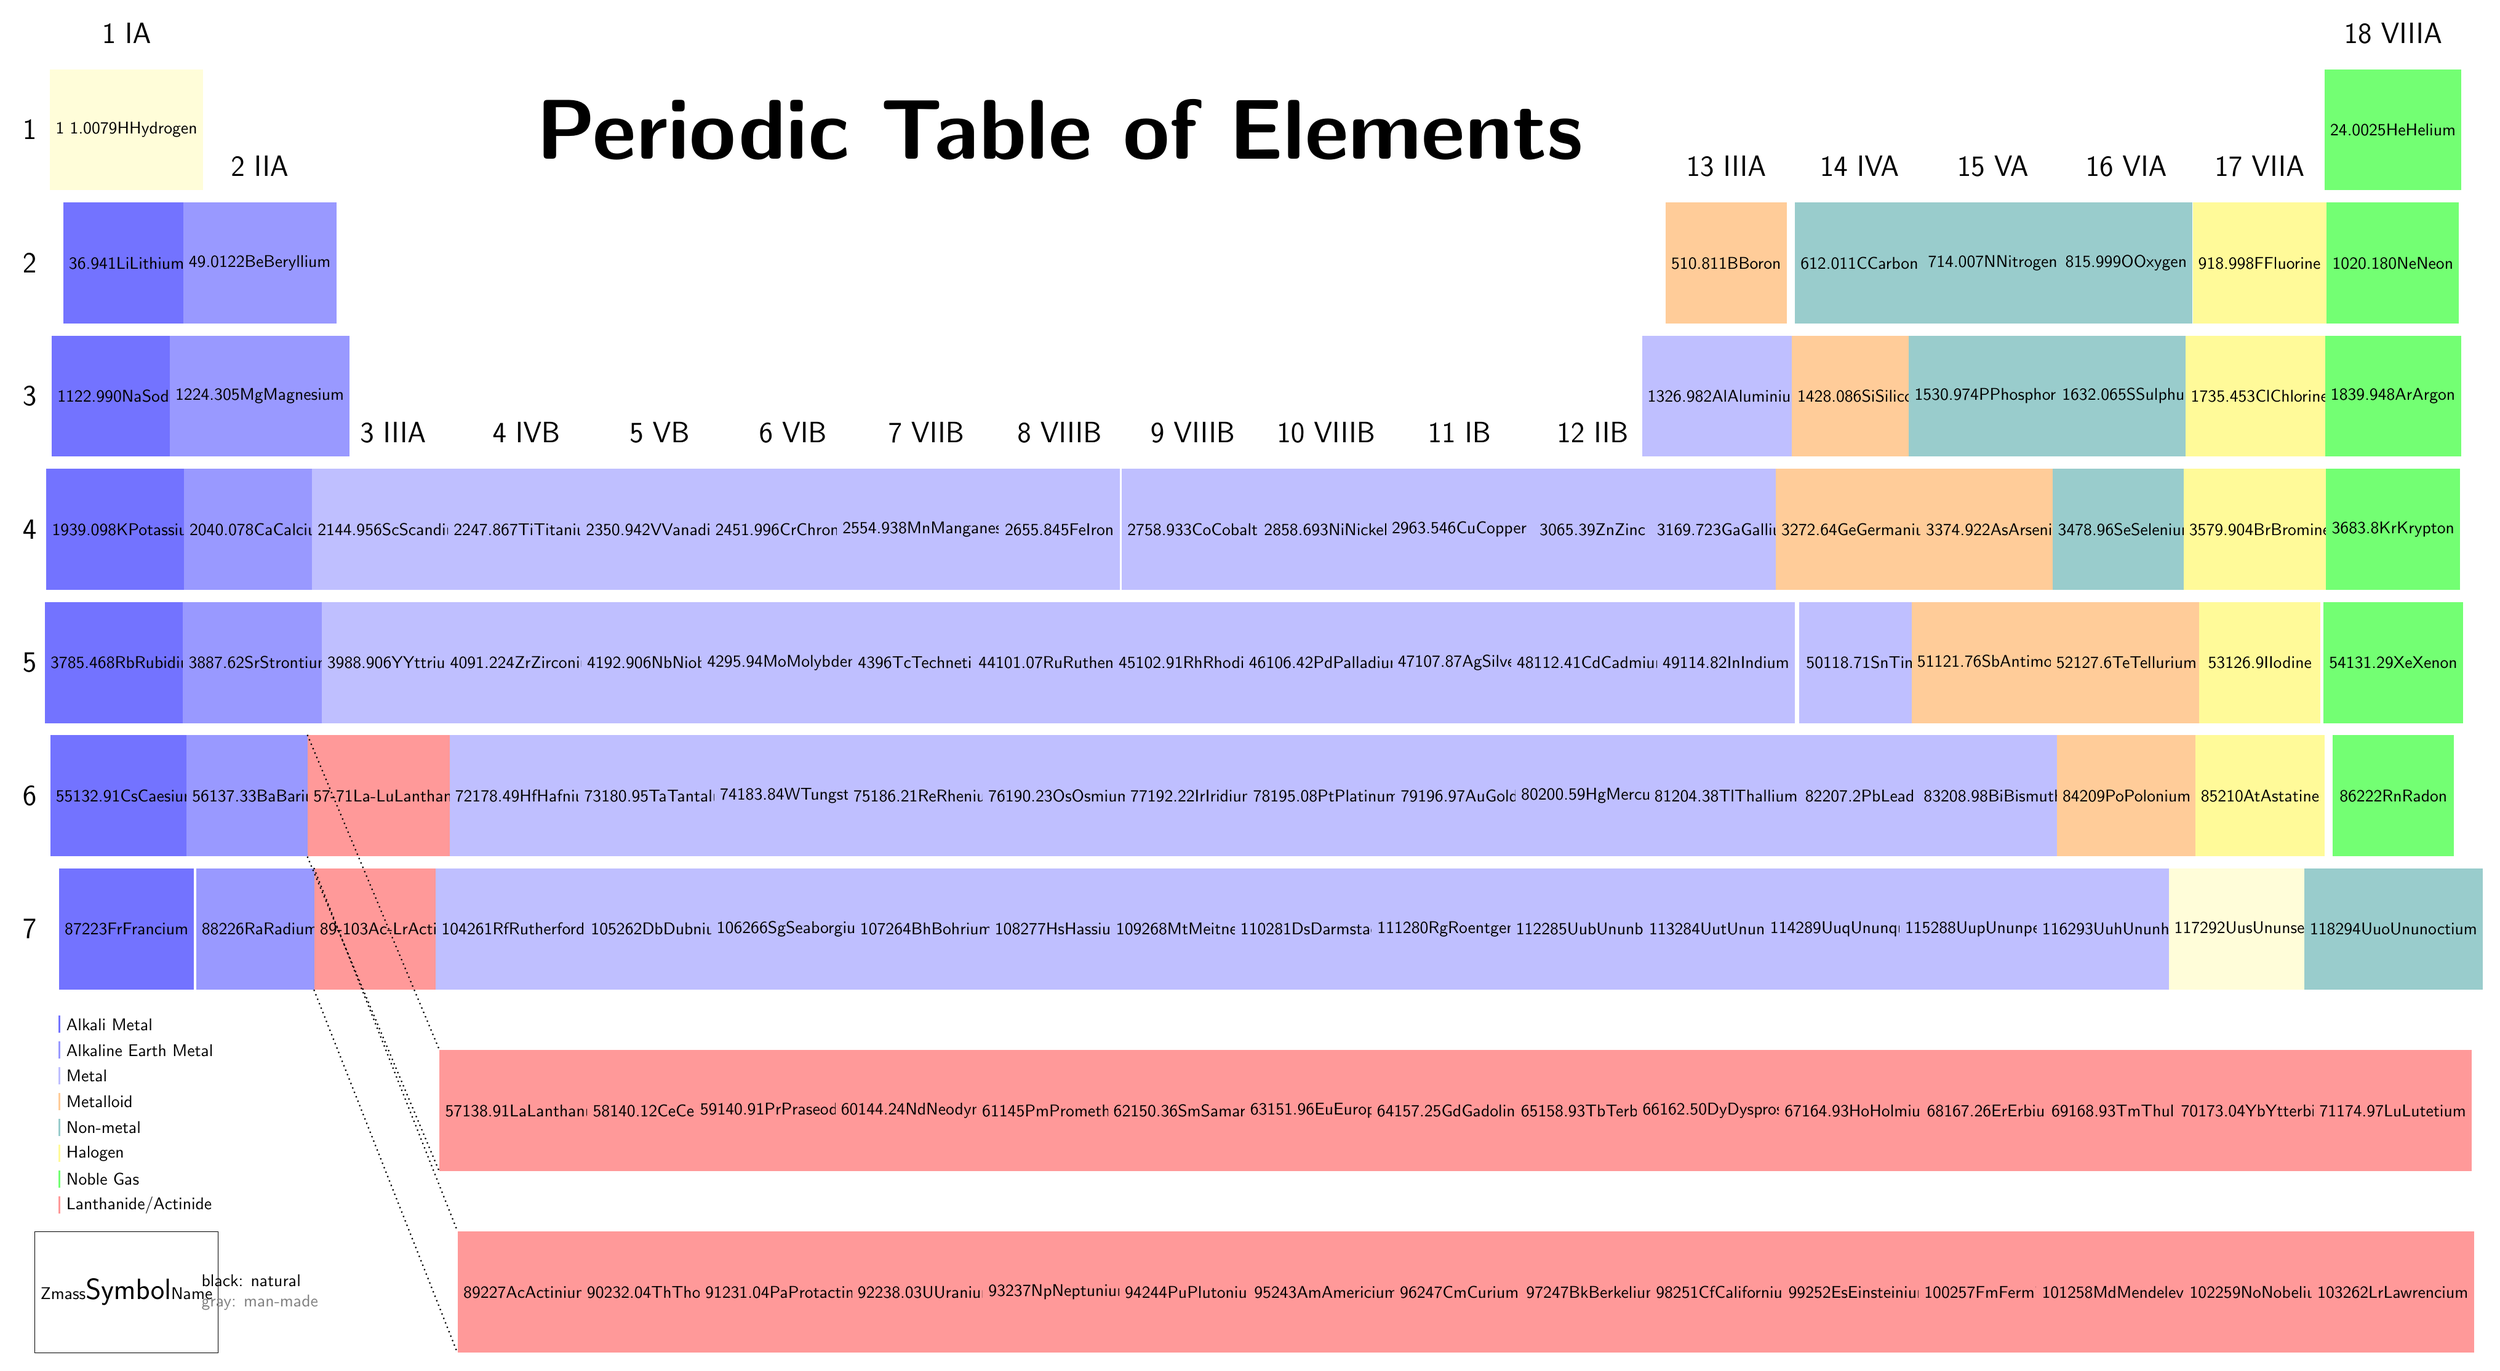
\begin{tikzpicture}[font=\sffamily,xscale=0.1]
	
	% Fill Color Styles
	\tikzstyle{ElementFill} = [fill=yellow!15]
	\tikzstyle{AlkaliMetalFill} = [fill=blue!55]
	\tikzstyle{AlkalineEarthMetalFill} = [fill=blue!40]
	\tikzstyle{MetalFill} = [fill=blue!25]
	\tikzstyle{MetalloidFill} = [fill=orange!40]
	\tikzstyle{NonmetalFill} = [fill=teal!40]
	\tikzstyle{HalogenFill} = [fill=yellow!40]
	\tikzstyle{NobleGasFill} = [fill=green!55]
	\tikzstyle{LanthanideActinideFill} = [fill=red!40]
	
	% Element Styles
	\tikzstyle{Element} = [ElementFill,
	minimum width=2.5cm, minimum height=2.5cm, node distance=2.75cm]
	\tikzstyle{AlkaliMetal} = [Element, AlkaliMetalFill]
	\tikzstyle{AlkalineEarthMetal} = [Element, AlkalineEarthMetalFill]
	\tikzstyle{Metal} = [Element, MetalFill]
	\tikzstyle{Metalloid} = [Element, MetalloidFill]
	\tikzstyle{Nonmetal} = [Element, NonmetalFill]
	\tikzstyle{Halogen} = [Element, HalogenFill]
	\tikzstyle{NobleGas} = [Element, NobleGasFill]
	\tikzstyle{LanthanideActinide} = [Element, LanthanideActinideFill]
	\tikzstyle{PeriodLabel} = [font={\sffamily\LARGE}, node distance=2.0cm]
	\tikzstyle{GroupLabel} = [font={\sffamily\LARGE}, minimum width=2.75cm, node distance=2.0cm]
	
	% Group 1 - IA
	\node[Element] (H) {\NaturalElem{1} {1.0079}{H}{Hydrogen}};
	\node[below of=H, AlkaliMetal] (Li) {\NaturalElem{3}{6.941}{Li}{Lithium}};
	\node[below of=Li, AlkaliMetal] (Na) {\NaturalElem{11}{22.990}{Na}{Sodium}};
	\node[below of=Na, AlkaliMetal] (K) {\NaturalElem{19}{39.098}{K}{Potassium}};
	\node[below of=K, AlkaliMetal] (Rb) {\NaturalElem{37}{85.468}{Rb}{Rubidium}};
	\node[below of=Rb, AlkaliMetal] (Cs) {\NaturalElem{55}{132.91}{Cs}{Caesium}};
	\node[below of=Cs, AlkaliMetal] (Fr) {\NaturalElem{87}{223}{Fr}{Francium}};
	
	% Group 2 - IIA
	\node[right of=Li, AlkalineEarthMetal] (Be) {\NaturalElem{4}{9.0122}{Be}{Beryllium}};
	\node[below of=Be, AlkalineEarthMetal] (Mg) {\NaturalElem{12}{24.305}{Mg}{Magnesium}};
	\node[below of=Mg, AlkalineEarthMetal] (Ca) {\NaturalElem{20}{40.078}{Ca}{Calcium}};
	\node[below of=Ca, AlkalineEarthMetal] (Sr) {\NaturalElem{38}{87.62}{Sr}{Strontium}};
	\node[below of=Sr, AlkalineEarthMetal] (Ba) {\NaturalElem{56}{137.33}{Ba}{Barium}};
	\node[below of=Ba, AlkalineEarthMetal] (Ra) {\NaturalElem{88}{226}{Ra}{Radium}};
	
	% Group 3 - IIIB
	\node[right of=Ca, Metal] (Sc) {\NaturalElem{21}{44.956}{Sc}{Scandium}};
	\node[below of=Sc, Metal] (Y) {\NaturalElem{39}{88.906}{Y}{Yttrium}};
	\node[below of=Y, LanthanideActinide] (LaLu) {\NaturalElem{57-71}{}{La-Lu}{Lanthanide}};
	\node[below of=LaLu, LanthanideActinide] (AcLr) {\NaturalElem{89-103}{}{Ac-Lr}{Actinide}};
	
	% Group 4 - IVB
	\node[right of=Sc, Metal] (Ti) {\NaturalElem{22}{47.867}{Ti}{Titanium}};
	\node[below of=Ti, Metal] (Zr) {\NaturalElem{40}{91.224}{Zr}{Zirconium}};
	\node[below of=Zr, Metal] (Hf) {\NaturalElem{72}{178.49}{Hf}{Hafnium}};
	\node[below of=Hf, Metal] (Rf) {\SyntheticElem{104}{261}{Rf}{Rutherfordium}};
	
	% Group 5 - VB
	\node[right of=Ti, Metal] (V) {\NaturalElem{23}{50.942}{V}{Vanadium}};
	\node[below of=V, Metal] (Nb) {\NaturalElem{41}{92.906}{Nb}{Niobium}};
	\node[below of=Nb, Metal] (Ta) {\NaturalElem{73}{180.95}{Ta}{Tantalum}};
	\node[below of=Ta, Metal] (Db) {\SyntheticElem{105}{262}{Db}{Dubnium}};
	
	% Group 6 - VIB
	\node[right of=V, Metal] (Cr) {\NaturalElem{24}{51.996}{Cr}{Chromium}};
	\node[below of=Cr, Metal] (Mo) {\NaturalElem{42}{95.94}{Mo}{Molybdenum}};
	\node[below of=Mo, Metal] (W) {\NaturalElem{74}{183.84}{W}{Tungsten}};
	\node[below of=W, Metal] (Sg) {\SyntheticElem{106}{266}{Sg}{Seaborgium}};
	
	% Group 7 - VIIB
	\node[right of=Cr, Metal] (Mn) {\NaturalElem{25}{54.938}{Mn}{Manganese}};
	\node[below of=Mn, Metal] (Tc) {\NaturalElem{43}{96}{Tc}{Technetium}};
	\node[below of=Tc, Metal] (Re) {\NaturalElem{75}{186.21}{Re}{Rhenium}};
	\node[below of=Re, Metal] (Bh) {\SyntheticElem{107}{264}{Bh}{Bohrium}};
	
	% Group 8 - VIIIB
	\node[right of=Mn, Metal] (Fe) {\NaturalElem{26}{55.845}{Fe}{Iron}};
	\node[below of=Fe, Metal] (Ru) {\NaturalElem{44}{101.07}{Ru}{Ruthenium}};
	\node[below of=Ru, Metal] (Os) {\NaturalElem{76}{190.23}{Os}{Osmium}};
	\node[below of=Os, Metal] (Hs) {\SyntheticElem{108}{277}{Hs}{Hassium}};
	
	% Group 9 - VIIIB
	\node[right of=Fe, Metal] (Co) {\NaturalElem{27}{58.933}{Co}{Cobalt}};
	\node[below of=Co, Metal] (Rh) {\NaturalElem{45}{102.91}{Rh}{Rhodium}};
	\node[below of=Rh, Metal] (Ir) {\NaturalElem{77}{192.22}{Ir}{Iridium}};
	\node[below of=Ir, Metal] (Mt) {\SyntheticElem{109}{268}{Mt}{Meitnerium}};
	
	% Group 10 - VIIIB
	\node[right of=Co, Metal] (Ni) {\NaturalElem{28}{58.693}{Ni}{Nickel}};
	\node[below of=Ni, Metal] (Pd) {\NaturalElem{46}{106.42}{Pd}{Palladium}};
	\node[below of=Pd, Metal] (Pt) {\NaturalElem{78}{195.08}{Pt}{Platinum}};
	\node[below of=Pt, Metal] (Ds) {\SyntheticElem{110}{281}{Ds}{Darmstadtium}};
	
	% Group 11 - IB
	\node[right of=Ni, Metal] (Cu) {\NaturalElem{29}{63.546}{Cu}{Copper}};
	\node[below of=Cu, Metal] (Ag) {\NaturalElem{47}{107.87}{Ag}{Silver}};
	\node[below of=Ag, Metal] (Au) {\NaturalElem{79}{196.97}{Au}{Gold}};
	\node[below of=Au, Metal] (Rg) {\SyntheticElem{111}{280}{Rg}{Roentgenium}};
	
	% Group 12 - IIB
	\node[right of=Cu, Metal] (Zn) {\NaturalElem{30}{65.39}{Zn}{Zinc}};
	\node[below of=Zn, Metal] (Cd) {\NaturalElem{48}{112.41}{Cd}{Cadmium}};
	\node[below of=Cd, Metal] (Hg) {\NaturalElem{80}{200.59}{Hg}{Mercury}};
	\node[below of=Hg, Metal] (Uub) {\SyntheticElem{112}{285}{Uub}{Ununbium}};
	
	% Group 13 - IIIA
	\node[right of=Zn, Metal] (Ga) {\NaturalElem{31}{69.723}{Ga}{Gallium}};
	\node[above of=Ga, Metal] (Al) {\NaturalElem{13}{26.982}{Al}{Aluminium}};
	\node[above of=Al, Metalloid] (B) {\NaturalElem{5}{10.811}{B}{Boron}};
	\node[below of=Ga, Metal] (In) {\NaturalElem{49}{114.82}{In}{Indium}};
	\node[below of=In, Metal] (Tl) {\NaturalElem{81}{204.38}{Tl}{Thallium}};
	\node[below of=Tl, Metal] (Uut) {\SyntheticElem{113}{284}{Uut}{Ununtrium}};
	
	% Group 14 - IVA
	\node[right of=B, Nonmetal] (C) {\NaturalElem{6}{12.011}{C}{Carbon}};
	\node[below of=C, Metalloid] (Si) {\NaturalElem{14}{28.086}{Si}{Silicon}};
	\node[below of=Si, Metalloid] (Ge) {\NaturalElem{32}{72.64}{Ge}{Germanium}};
	\node[below of=Ge, Metal] (Sn) {\NaturalElem{50}{118.71}{Sn}{Tin}};
	\node[below of=Sn, Metal] (Pb) {\NaturalElem{82}{207.2}{Pb}{Lead}};
	\node[below of=Pb, Metal] (Uuq) {\SyntheticElem{114}{289}{Uuq}{Ununquadium}};
	
	% Group 15 - VA
	\node[right of=C, Nonmetal] (N) {\NaturalElem{7}{14.007}{N}{Nitrogen}};
	\node[below of=N, Nonmetal] (P) {\NaturalElem{15}{30.974}{P}{Phosphorus}};
	\node[below of=P, Metalloid] (As) {\NaturalElem{33}{74.922}{As}{Arsenic}};
	\node[below of=As, Metalloid] (Sb) {\NaturalElem{51}{121.76}{Sb}{Antimony}};
	\node[below of=Sb, Metal] (Bi) {\NaturalElem{83}{208.98}{Bi}{Bismuth}};
	\node[below of=Bi, Metal] (Uup) {\SyntheticElem{115}{288}{Uup}{Ununpentium}};
	
	% Group 16 - VIA
	\node[right of=N, Nonmetal] (O) {\NaturalElem{8}{15.999}{O}{Oxygen}};
	\node[below of=O, Nonmetal] (S) {\NaturalElem{16}{32.065}{S}{Sulphur}};
	\node[below of=S, Nonmetal] (Se) {\NaturalElem{34}{78.96}{Se}{Selenium}};
	\node[below of=Se, Metalloid] (Te) {\NaturalElem{52}{127.6}{Te}{Tellurium}};
	\node[below of=Te, Metalloid] (Po) {\NaturalElem{84}{209}{Po}{Polonium}};
	\node[below of=Po, Metal] (Uuh) {\SyntheticElem{116}{293}{Uuh}{Ununhexium}};
	
	% Group 17 - VIIA
	\node[right of=O, Halogen] (F) {\NaturalElem{9}{18.998}{F}{Fluorine}};
	\node[below of=F, Halogen] (Cl) {\NaturalElem{17}{35.453}{Cl}{Chlorine}};
	\node[below of=Cl, Halogen] (Br) {\NaturalElem{35}{79.904}{Br}{Bromine}};
	\node[below of=Br, Halogen] (I) {\NaturalElem{53}{126.9}{I}{Iodine}};
	\node[below of=I, Halogen] (At) {\NaturalElem{85}{210}{At}{Astatine}};
	\node[below of=At, Element] (Uus) {\SyntheticElem{117}{292}{Uus}{Ununseptium}};
	
	% Group 18 - VIIIA
	\node[right of=F, NobleGas] (Ne) {\NaturalElem{10}{20.180}{Ne}{Neon}};
	\node[above of=Ne, NobleGas] (He) {\NaturalElem{2}{4.0025}{He}{Helium}};
	\node[below of=Ne, NobleGas] (Ar) {\NaturalElem{18}{39.948}{Ar}{Argon}};
	\node[below of=Ar, NobleGas] (Kr) {\NaturalElem{36}{83.8}{Kr}{Krypton}};
	\node[below of=Kr, NobleGas] (Xe) {\NaturalElem{54}{131.29}{Xe}{Xenon}};
	\node[below of=Xe, NobleGas] (Rn) {\NaturalElem{86}{222}{Rn}{Radon}};
	\node[below of=Rn, Nonmetal] (Uuo) {\SyntheticElem{118}{294}{Uuo}{Ununoctium}};
	
	% Period
	\node[left of=H, PeriodLabel] (Period1) {1};
	\node[left of=Li, PeriodLabel] (Period2) {2};
	\node[left of=Na, PeriodLabel] (Period3) {3};
	\node[left of=K, PeriodLabel] (Period4) {4};
	\node[left of=Rb, PeriodLabel] (Period5) {5};
	\node[left of=Cs, PeriodLabel] (Period6) {6};
	\node[left of=Fr, PeriodLabel] (Period7) {7};
	
	% Group
	\node[above of=H, GroupLabel] (Group1) {1 \hfill IA};
	\node[above of=Be, GroupLabel] (Group2) {2 \hfill IIA};
	\node[above of=Sc, GroupLabel] (Group3) {3 \hfill IIIA};
	\node[above of=Ti, GroupLabel] (Group4) {4 \hfill IVB};
	\node[above of=V, GroupLabel] (Group5) {5 \hfill VB};
	\node[above of=Cr, GroupLabel] (Group6) {6 \hfill VIB};
	\node[above of=Mn, GroupLabel] (Group7) {7 \hfill VIIB};
	\node[above of=Fe, GroupLabel] (Group8) {8 \hfill VIIIB};
	\node[above of=Co, GroupLabel] (Group9) {9 \hfill VIIIB};
	\node[above of=Ni, GroupLabel] (Group10) {10 \hfill VIIIB};
	\node[above of=Cu, GroupLabel] (Group11) {11 \hfill IB};
	\node[above of=Zn, GroupLabel] (Group12) {12 \hfill IIB};
	\node[above of=B, GroupLabel] (Group13) {13 \hfill IIIA};
	\node[above of=C, GroupLabel] (Group14) {14 \hfill IVA};
	\node[above of=N, GroupLabel] (Group15) {15 \hfill VA};
	\node[above of=O, GroupLabel] (Group16) {16 \hfill VIA};
	\node[above of=F, GroupLabel] (Group17) {17 \hfill VIIA};
	\node[above of=He, GroupLabel] (Group18) {18 \hfill VIIIA};
	
	% Lanthanide
	\node[below of=Rf, LanthanideActinide, yshift=-1cm] (La) {\NaturalElem{57}{138.91}{La}{Lanthanum}};
	\node[right of=La, LanthanideActinide] (Ce) {\NaturalElem{58}{140.12}{Ce}{Cerium}};
	\node[right of=Ce, LanthanideActinide] (Pr) {\NaturalElem{59}{140.91}{Pr}{Praseodymium}};
	\node[right of=Pr, LanthanideActinide] (Nd) {\NaturalElem{60}{144.24}{Nd}{Neodymium}};
	\node[right of=Nd, LanthanideActinide] (Pm) {\NaturalElem{61}{145}{Pm}{Promethium}};
	\node[right of=Pm, LanthanideActinide] (Sm) {\NaturalElem{62}{150.36}{Sm}{Samarium}};
	\node[right of=Sm, LanthanideActinide] (Eu) {\NaturalElem{63}{151.96}{Eu}{Europium}};
	\node[right of=Eu, LanthanideActinide] (Gd) {\NaturalElem{64}{157.25}{Gd}{Gadolinium}};
	\node[right of=Gd, LanthanideActinide] (Tb) {\NaturalElem{65}{158.93}{Tb}{Terbium}};
	\node[right of=Tb, LanthanideActinide] (Dy) {\NaturalElem{66}{162.50}{Dy}{Dysprosium}};
	\node[right of=Dy, LanthanideActinide] (Ho) {\NaturalElem{67}{164.93}{Ho}{Holmium}};
	\node[right of=Ho, LanthanideActinide] (Er) {\NaturalElem{68}{167.26}{Er}{Erbium}};
	\node[right of=Er, LanthanideActinide] (Tm) {\NaturalElem{69}{168.93}{Tm}{Thulium}};
	\node[right of=Tm, LanthanideActinide] (Yb) {\NaturalElem{70}{173.04}{Yb}{Ytterbium}};
	\node[right of=Yb, LanthanideActinide] (Lu) {\NaturalElem{71}{174.97}{Lu}{Lutetium}};
	
	% Actinide
	\node[below of=La, LanthanideActinide, yshift=-1cm] (Ac) {\NaturalElem{89}{227}{Ac}{Actinium}};
	\node[right of=Ac, LanthanideActinide] (Th) {\NaturalElem{90}{232.04}{Th}{Thorium}};
	\node[right of=Th, LanthanideActinide] (Pa) {\NaturalElem{91}{231.04}{Pa}{Protactinium}};
	\node[right of=Pa, LanthanideActinide] (U) {\NaturalElem{92}{238.03}{U}{Uranium}};
	\node[right of=U, LanthanideActinide] (Np) {\SyntheticElem{93}{237}{Np}{Neptunium}};
	\node[right of=Np, LanthanideActinide] (Pu) {\SyntheticElem{94}{244}{Pu}{Plutonium}};
	\node[right of=Pu, LanthanideActinide] (Am) {\SyntheticElem{95}{243}{Am}{Americium}};
	\node[right of=Am, LanthanideActinide] (Cm) {\SyntheticElem{96}{247}{Cm}{Curium}};
	\node[right of=Cm, LanthanideActinide] (Bk) {\SyntheticElem{97}{247}{Bk}{Berkelium}};
	\node[right of=Bk, LanthanideActinide] (Cf) {\SyntheticElem{98}{251}{Cf}{Californium}};
	\node[right of=Cf, LanthanideActinide] (Es) {\SyntheticElem{99}{252}{Es}{Einsteinium}};
	\node[right of=Es, LanthanideActinide] (Fm) {\SyntheticElem{100}{257}{Fm}{Fermium}};
	\node[right of=Fm, LanthanideActinide] (Md) {\SyntheticElem{101}{258}{Md}{Mendelevium}};
	\node[right of=Md, LanthanideActinide] (No) {\SyntheticElem{102}{259}{No}{Nobelium}};
	\node[right of=No, LanthanideActinide] (Lr) {\SyntheticElem{103}{262}{Lr}{Lawrencium}};
	
	% Draw dotted lines connecting Lanthanide breakout to main table
	\draw[thick,dotted] (LaLu.north west) -- (La.north west)
	(LaLu.south west) -- (La.south west);
	% Draw dotted lines connecting Actinide breakout to main table
	\draw[thick,dotted] (AcLr.north west) -- (Ac.north west)
	(AcLr.south west) -- (Ac.south west);
	
	% Legend
	\fill[AlkaliMetalFill] ($(La.north -| Fr.west) + (0,1em)$)
	rectangle +(1em, 1em) node[right, yshift=-1.2ex]  (AlkaliMetal) {Alkali Metal};
	\fill[AlkalineEarthMetalFill] ($(AlkaliMetal.west) - (1em,2em)$)
	rectangle +(1em, 1em) node[right, yshift=-1.2ex] (AlkalineEarthMetal) {Alkaline Earth Metal};
	\fill[MetalFill] ($(AlkalineEarthMetal.west) - (1em,2em)$)
	rectangle +(1em, 1em) node[right, yshift=-1.2ex] (Metal) {Metal};
	\fill[MetalloidFill] ($(Metal.west) - (1em,2em)$)
	rectangle +(1em, 1em) node[right, yshift=-1.2ex] (Metalloid) {Metalloid};
	\fill[NonmetalFill] ($(Metalloid.west) - (1em,2em)$)
	rectangle +(1em, 1em) node[right, yshift=-1.2ex] (Non-metal) {Non-metal};
	\fill[HalogenFill] ($(Non-metal.west) - (1em,2em)$)
	rectangle +(1em, 1em) node[right, yshift=-1.2ex] (Halogen) {Halogen};
	\fill[NobleGasFill] ($(Halogen.west) - (1em,2em)$)
	rectangle +(1em, 1em) node[right, yshift=-1.2ex] (NobleGas) {Noble Gas};
	\fill[LanthanideActinideFill] ($(NobleGas.west) - (1em,2em)$)
	rectangle +(1em, 1em) node[right, yshift=-1.2ex] (Lanthanide/Actinide) {Lanthanide/Actinide};
	
	\node at (Ac -| Fr) [draw, Element, fill=white] (legend) {\NaturalElem{Z}{mass}{\LARGE Symbol}{Name}};
	\node[align=left] at (Ac -| Ra) {black: natural\\\color{gray}gray: man-made};
	
	% Diagram Title
	\node at (H.west -| Fe.north) [scale=2, font={\sffamily\Huge\bfseries}]
	{Periodic Table of Elements};
	
\end{tikzpicture}
\end{landscape}
\end{document}
